\section{Decay with Decay Partners at Different Distances}

\begin{figure}[h]
 \centering
 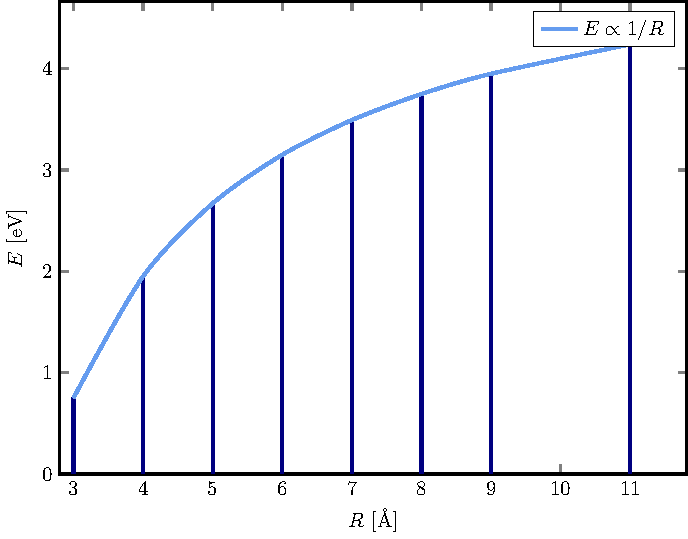
\includegraphics[width=\columnwidth]{pics/model_RE.pdf}
 \caption{Kinetic energy of the ICD electron depending on the interatomic
          distance of the two atoms involved in the decay within the
          asymptotic approximation. The kinetic energy shows a $1/R$
          behaviour and hence distance changes at small distances lead
          to larger changes in the kinetic energy than at larger distances.}
 \label{figure:model_RE}
\end{figure}


\begin{figure}[h]
 \centering
 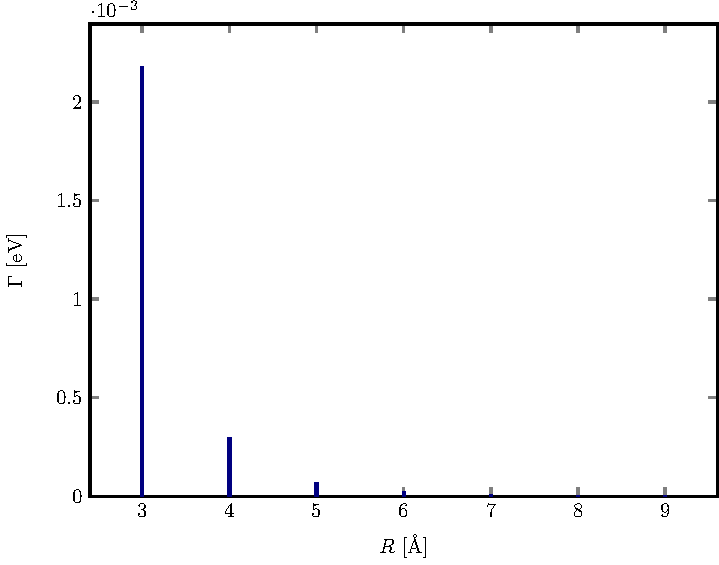
\includegraphics[width=\columnwidth]{pics/model_RGamma.pdf}
 \caption{Decay widths for different interatomic distances following an
          asymptotic $1/R^6$-behaviour. For distances larger than twice
          the shortest distance considered the peaks are not visible in this
          plot.}
 \label{figure:model_RGamma}
\end{figure}

\begin{figure}[h]
 \centering
 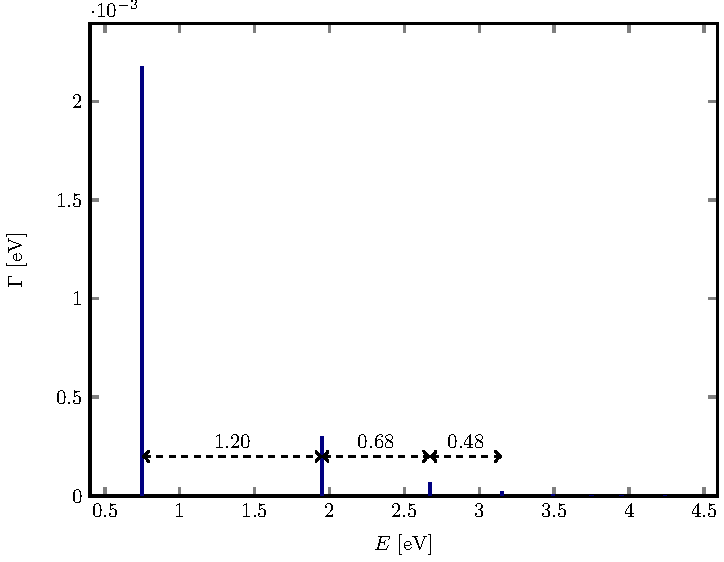
\includegraphics[width=\columnwidth]{pics/model_EGamma.pdf}
 \caption{ICD electron spectrum for interaction partner distances of
          \unit[3]{\AA}, \unit[4]{\AA}, \unit[5]{\AA}, \dots ,\unit[11]{\AA}.
          The energy difference between equidistant interaction partners
          decreases with increasing distance. For the case of Ne$_2$ pairs
          these energy differences between the peaks stemming from different
          interatomic distances are given by:
          \unit[3]{\AA},\unit[4]{\AA} $\rightarrow$ \unit[1.20]{eV},
          \unit[4]{\AA},\unit[5]{\AA} $\rightarrow$ \unit[0.68]{eV} and
          \unit[5]{\AA},\unit[6]{\AA} $\rightarrow$ \unit[0.48]{eV}.
          This means that the spectrum is better resolved for smaller distances
          and that small distance changes like vibrations will mainly affect
          this lower energy part of the spectrum.
}
 \label{figure:model_EGamma}
\end{figure}



%\begin{figure}
% \centering
% \includegraphics[width=\textwidth]{pics/}
% \caption{}
% \label{}
%\end{figure}
